\section{Identificazione e delimitazione del bacino idrografico sede dell'intervento}
Il bacino idrografico d'interesse per questa relazione è quello relativo al torrente Sigismondi, con punto di chiusura a INSERIRE PUNTO CHIUSURA\\
Al fine di individuare il bacino idrografico del punto considerato sulla CTP (Carta Tecnica Provinciale), è necessario delineare la linea spartiacque.\\
Per fare ciò, occorre tenere in considerazione l'andamento delle creste dei versanti ed in cui l'acqua che vi scorre tenderà ad andare verso il punto di chiusura.\\
Fatto ciò, si analizzano gli elementi del reticolo idrografico interno al bacino; si attribuisce ad ogni ramo il proprio ordine, in base alla propria gerarchia. In base all'ordine del tratto coincidente con la sezione di chiusura, si attribuisce lo stesso ordine al bacino (questo verrà ripetuto successivamente).
\begin{figure}[H]\centering
    \includegraphics[scale=.40]{immagini/scan_ctp.pdf}
    \caption{Rappresentazione dello spartiacque e del reticolo idrografico del bacino di nostro interesse, nella CTP.}
  \label{scan_ctp}
\end{figure}

\noindent Un metodo alternativo a quello appena descritto, che necessita della cartografia tradizionale, è quello che implica l'utilizzo di un software GIS (Geographic information system).\\
Immettendo nel programma (Qgis nel nostro caso) il modello digitale del terreno (DTM) dell'area di nostro interesse, è possibile estrarre informazioni utili per l'analisi spaziale, come per esempio la lunghezza dello spartiacque, la superficie totale, etc.\\
Il DTM è semplificabile come un file raster (ovvero non vettoriale) che attribuisce ad ogni punto geografico del terreno (2 coordinate) la relativa quota altimetrica. Generalmente, tale modello viene prodotto partendo da rilievi svolti tramite foto-satelliti o sensori posti su droni; la loro fruizione è quasi spesso libera poiché vengono resi disponibili nei geoportali territoriali (Provincia di Trento in questo caso).\\
Quindi, partendo dal modello digitale del terreno dell'area d'interesse è possibile cominciare l'attività di analisi.\\
\begin{figure}[H]\centering
    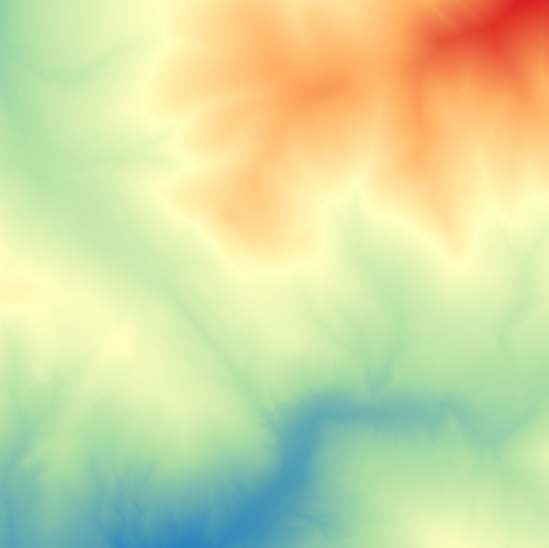
\includegraphics[scale=.50]{immagini/dtm_qgis.PNG}
    \caption{Rappresentazione del DTM dell'area di studio.}
    \label{dtm_qgis}
\end{figure}
\noindent Il software Qgis, per semplificare la visione della variazione di livello, permette di assegnare colori omogenei a punti con quote simili.\\ 
Durante la campagna di rilevamento dei punti, o nel successivo processo di analisi dei dati, inevitabilmente vengono a crearsi delle celle con depressioni locali, detti ``pits", ovvero errori. Questo fenomeno, anomalo nella realtà, viene modificato dal software GIS mediante un filtraggio (detto ``deppittaggio").\\
Successivamente a questa modifica, le quote altimetriche delle celle vengono analizzate, in modo da determinare la direzione di deflusso dell'acqua (\textit{flow direction}) verso la sezione di chiusura, secondo la massima pendenza verso valle.\\
In questo modo, è possibile conoscere per ogni cella la superficie drenante del bacino che la attraversa (\textit{upslope area}).\\
Per delimitare la rete idrografica del bacino, al fine di estrarre la mappa del bacino, è necessario porre un'area di soglia, ovvero la superficie minima drenante che ogni cella del bacino deve avere, al fine di essere considerata in questo processo.\\
Per estrarre il reticolo corretto, ovvero concorde con la CTP, è necessario svolgere dei tentativi; il compromesso migliore lo si trova imponendo un limite di area di 60000 $m^2$ (6 $ha$). Il reticolo idrografico estratto può essere osservato nella figura \ref{bacino_reticolo_qgis}.\\
Attraverso la determinazione della sezione di chiusura, nel nostro caso vincolata dal progetto, il software GIS permette di estrarre il bacino idrografico complessivo.\\
\begin{figure}[H]\centering
    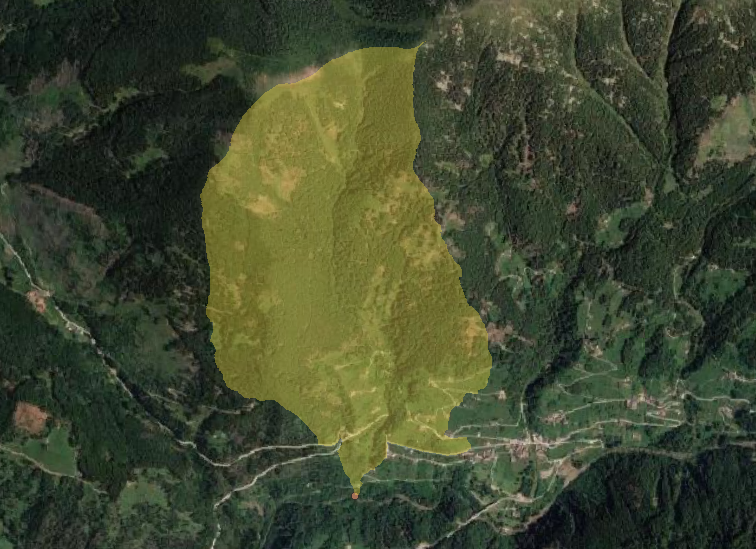
\includegraphics[scale=.50]{immagini/bacino_qgis.PNG}
    \caption{Rappresentazione del bacino idrografico e della sua sezione di chiusura.}
    \label{bacino_qgis}
\end{figure}
\noindent Per migliorare la visione, e comprendere meglio il territorio in analisi, è possibile simulare il fenomeno di ombreggiamento creato dal sole sui versanti e sulle valli.
\begin{figure}[H]\centering
    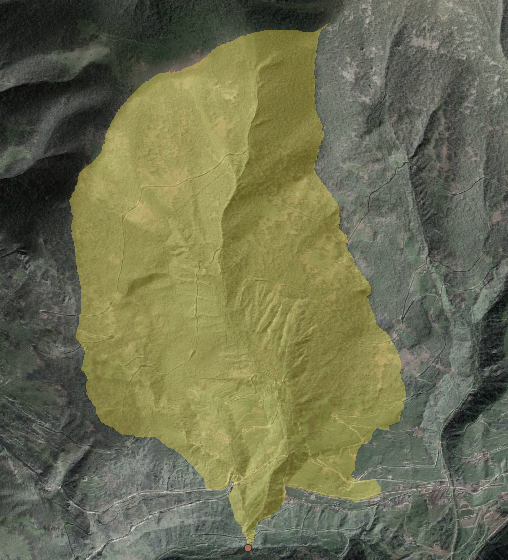
\includegraphics[scale=.50]{immagini/bacino_ombreggiatura_qgis.PNG}
    \caption{Rappresentazione del bacino idrografico, della sua sezione di chiusura e dell'effetto di ombreggiamento.}
    \label{bacino_ombreggiatura_qgis}
\end{figure}

\begin{figure}[H]
    \centering
    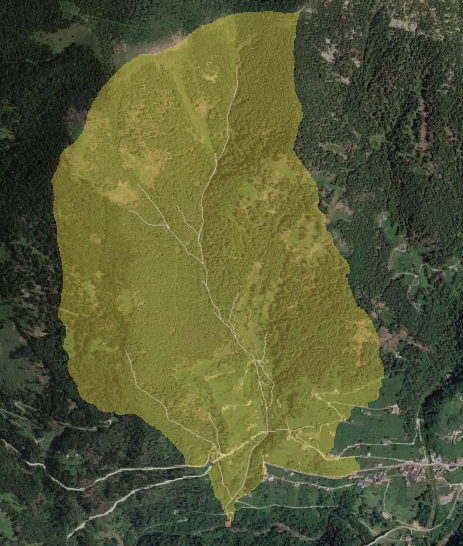
\includegraphics[scale=0.60]{immagini/bacino_reticolo_ombreg_qgis.PNG}
    \caption{Rappresentazione del bacino e del reticolo idrografico, con indicazione della sezione di chiusura.}
    \label{bacino_reticolo_qgis}
    \end{figure}

\noindent Dal reticolo idrografico di un bacino è possibile svolgere alcune considerazioni, come per esempio quella riguardante i suoi segmenti.\\
A seconda del numero di segmenti di cui è formato il reticolo, il bacino assume lo stesso valore di ordine, detto ``ordine del bacino" ed indicato con la lettera $k$.\\
Secondo il metodo di Horton-Strahler, l'attribuzione dell'ordine al segmento del reticolo idrografico avviene mediante tre regole: 
\begin{enumerate}
    \item ai tratti iniziali (di sorgente) viene attribuito valore 1;
    \item nel caso di confluenza di due tratti di diverso ordine, al segmento a valle viene attribuito il valore maggiore tra i due;
    \item nel caso di confluenza di due tratti con ordine $x$, al segmento a valle viene attribuito un valore $x+1$.
\end{enumerate} 
Avendo assegnato ad ogni tratto un certo valore numerico, è possibile conoscere la numerosità di ogni ordine.
\begin{figure}[H]\centering
    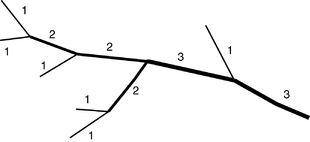
\includegraphics[scale=.75]{immagini/ordine_horton.png}
    \caption{Criterio di assegnazione dell'ordine ai segmenti del reticolo idrografico, secondo Horton-Strahler.}
  \label{ordine_horton}
\end{figure}
 
\paragraph{Reticolo idrografico secondo la CTP}
Nel caso di studio mediante l'utilizzo della Carta Tecnica Provinciale (\ref{scan_ctp}), il reticolo idrografico del bacino è formato da un'asta principale e da quattro tratti laterali, disposti sulla destra idraulica di quella maggiore.\\
Essendo che il segmento coincidente con il punto di chiusura possiede valore 3, di conseguenza l'intero bacino idrologico è di ordine 3.\\
La frequenza degli ordini dei segmenti è la seguente:
\begin{table}[H] \centering
    \begin{tabular}{cc}
\toprule
    Ordine u & Segmenti Nu \\
\midrule    
    1        & 5           \\
    2        & 2           \\
    3        & 1           \\
\bottomrule    
\end{tabular}
\end{table}
\paragraph{Reticolo idrografico secondo il DTM}
Studiando il reticolo idrografico generato dal DTM (\ref{bacino_reticolo_qgis}), si può osservare un maggiore numero di segmenti di ordine primo.\\
Anche in questo caso, l'ordine del bacino è di ordine 3.\\
La frequenza degli ordini dei segmenti è la seguente:
\begin{table}[H] \centering
    \begin{tabular}{cc}
\toprule
    Ordine u & Segmenti Nu \\
\midrule    
    1        & 12          \\
    2        & 3          \\
    3        & 1           \\
\bottomrule    
\end{tabular}
\end{table}

\subsection{Ulteriori caratteristiche del bacino}
\begin{figure}[H] 
    \begin{minipage}[]{7cm}
        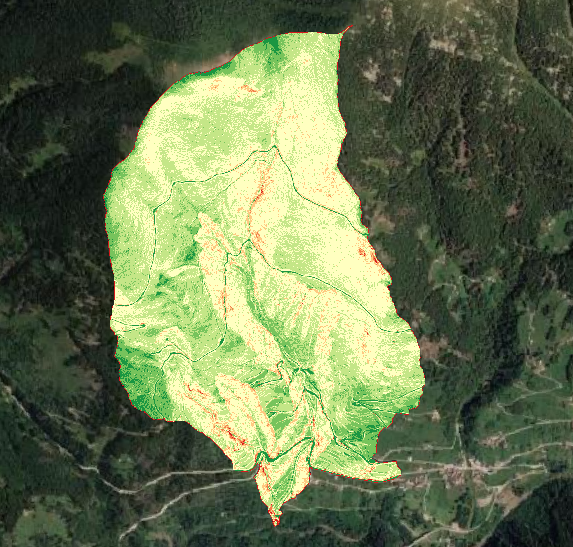
\includegraphics[scale=0.58]{immagini/bacino_slope.PNG}
        \caption{Rappresentazione della pendenza dei versanti del bacino.}
        \end{minipage}
        \hspace{2cm}
    \begin{minipage}[]{7cm}
        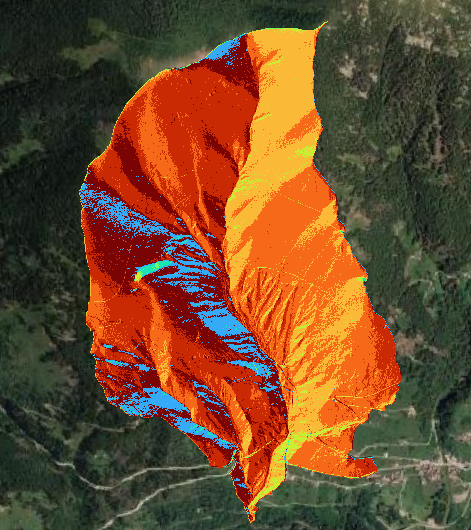
\includegraphics[scale=0.6]{immagini/bacino_orientamento_qgis.PNG}
        \caption{Orientamento dei versanti del bacino idrografico.}
    \end{minipage} 
        \end{figure}
       
\begin{figure}[H]  \centering
        \begin{minipage}[]{7cm}	
            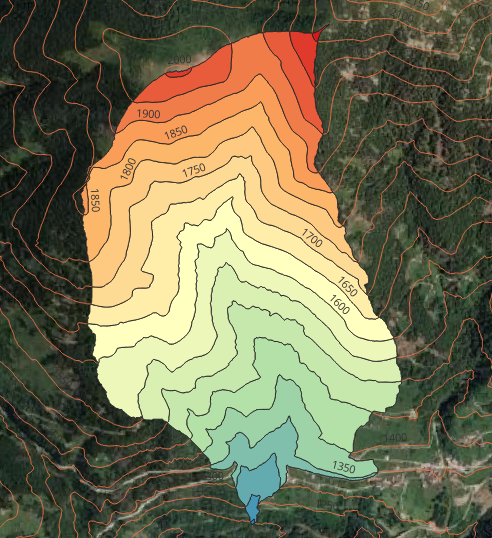
\includegraphics[scale=0.6]{immagini/bacino_fasce_quota_qgis.PNG}
        \caption{Rappresentazione delle fasce di quota altimetrica del bacino.}
        \end{minipage}  
\end{figure}
